\section{Results}
\label{sec:results}

\subsection{Effectiveness of the learned policy: RLTabucol vs. RLTabucol$_0$ and Pure Tabucol}
\label{ssec:res-default}

Table 2 compares RLTabucol with its random-policy baseline RLTabucol$_0$ and standalone Pure Tabucol. Against the matched random-policy control RLTabucol$_0$, RLTabucol matches or improves the achieved $k_{\mathrm{best}}$ on 8 of 11 instances: it reaches a lower $k_{\mathrm{best}}$ on four, ties on four, and requires one additional color on three. The largest reductions are two colors on \texttt{DSJC500.9} and three colors on \texttt{flat1000\_76\_0}. At the same time, the three failures show that the learned guidance is not uniformly beneficial. The policy is therefore clearly different from random recoloring and proved useful, but its value is non-universal across test instances

The comparison with Pure Tabucol tests more directly whether adding the learned policy improves the final graph-coloring solution quality over traditional Tabucol to achieve the goal of optimization. Both methods receive the same five-hour wall-clock budget. However, pure Tabucol spends this budget entirely on local search, whereas RLTabucol divides it between actor inference and repeated Tabucol calls. RLTabucol lowers $k_{\mathrm{best}}$ only on \texttt{flat1000\_76\_0} ($87$ versus $88$), ties Pure Tabucol on nine instances, and is worse on \texttt{flat300\_28\_0} ($31$ versus $30$). At tied color budgets, timing and success are also mixed. On \texttt{DSJC500.1}, for example, RLTabucol reaches $k=12$ in $8/10$ runs and has a lower best and mean successful-run time than Pure Tabucol, whereas on \texttt{DSJC500.5} it succeeds in only $6/10$ runs at $k=49$, compared with $10/10$ for Pure Tabucol. Thus, RLTabucol shows that the learned policy can be useful, but the RLTabucol framework does not yet consistently surpass Pure Tabucol and therefore does not fully realize the intended optimization objective.

Taken together, the first between RLTabucol and RLTabucol$_0$ establishes that the learned policy carries useful search information, whereas the second comprison between RLTabucol and pure tabucol shows that RLTabucol itself is not yet a consistently stronger optimizer than Pure Tabucol. To further investigate the failure cases and the behavior of policy, the actor-only experiment in the next section therefore examines what the policy can achieve without Tabucol, how much fine repair Tabucol contributes, and whether their handoff is a plausible source of the remaining limitation.

\begin{table*}[t]
\centering
\caption{Comparison among Pure Tabucol, RLTabucol, and the random-policy baseline RLTabucol$_0$. Time reports best / mean wall-clock seconds over successful runs only. Bold $k_{\rm best}$ values are the lowest per row, including ties. Best and mean times are compared and bolded independently only among methods attaining the row-minimum color budget.}
\label{tab:rltabucol-default}
\setlength{\tabcolsep}{2.5pt}
\resizebox{\textwidth}{!}{\begin{tabular}{@{}lccccccccc@{}}
\toprule
Instance & \multicolumn{3}{c}{Pure Tabucol} & \multicolumn{3}{c}{RLTabucol} & \multicolumn{3}{c}{RLTabucol$_0$}\\
 & $k_{\rm best}$ & Success & Time (s) & $k_{\rm best}$ & Success & Time (s) & $k_{\rm best}$ & Success & Time (s)\\
\midrule
\texttt{DSJC250.5} & \textbf{28} & 10/10 & 14.6 / 45.5 & \textbf{28} & 10/10 & 243.8 / 3046.5 & \textbf{28} & 10/10 & \textbf{2.6} / \textbf{269.0} \\
\texttt{DSJC500.1} & \textbf{12} & 7/10 & 2356.2 / 6001.4 & \textbf{12} & 8/10 & \textbf{936.9} / \textbf{3616.9} & 13 & 10/10 & 0.4 / 0.6 \\
\texttt{DSJC500.5} & \textbf{49} & 10/10 & \textbf{408.5} / \textbf{1519.6} & \textbf{49} & 6/10 & 2375.5 / 7664.3 & 50 & 10/10 & 101.9 / 1303.2 \\
\texttt{DSJC500.9} & \textbf{128} & 8/10 & \textbf{2513.0} / \textbf{8521.6} & \textbf{128} & 4/10 & 3062.7 / 8749.3 & 130 & 7/10 & 1080.5 / 4289.1 \\
\texttt{le450\_15c} & 16 & 10/10 & 0.2 / 45.2 & 16 & 10/10 & 4.1 / 246.7 & \textbf{15} & 10/10 & \textbf{273.1} / \textbf{1283.2} \\
\texttt{le450\_15d} & 16 & 9/10 & 0.3 / 302.5 & 16 & 10/10 & 32.2 / 1085.3 & \textbf{15} & 9/10 & \textbf{932.4} / \textbf{6956.8} \\
\texttt{le450\_25c} & \textbf{26} & 9/10 & 5.4 / 12.4 & \textbf{26} & 10/10 & 44.7 / 141.0 & \textbf{26} & 10/10 & \textbf{3.3} / \textbf{16.5} \\
\texttt{le450\_25d} & \textbf{26} & 10/10 & 7.6 / 14.5 & \textbf{26} & 10/10 & 44.8 / 106.6 & \textbf{26} & 10/10 & \textbf{1.9} / \textbf{17.5} \\
\texttt{flat300\_26\_0} & \textbf{26} & 10/10 & \textbf{8.8} / \textbf{215.8} & \textbf{26} & 10/10 & 229.2 / 1147.8 & \textbf{26} & 10/10 & 134.3 / 704.4 \\
\texttt{flat300\_28\_0} & \textbf{30} & 1/10 & \textbf{9453.8} / \textbf{9453.8} & 31 & 10/10 & 150.4 / 1278.2 & \textbf{30} & 1/10 & 14021.1 / 14021.1 \\
\texttt{flat1000\_76\_0} & 88 & 1/10 & 16485.4 / 16485.4 & \textbf{87} & 1/10 & \textbf{8920.2} / \textbf{8920.2} & 90 & 10/10 & 303.9 / 1349.2 \\
\bottomrule
\end{tabular}
}
\end{table*}

\subsection{Actor-only analysis of the policy--Tabucol interface}
\label{ssec:res-actor}

We select \texttt{le450\_15d} as a representative failure case and examine
the actor's standalone behavior at $k=15$ in
Figure~\ref{fig:actor-only-curve}. Across ten complete actor-only runs, the best conflict counts at termination range from $203$ to $243$, with mean $225.5$ and median $223.5$. The ten complete diagnostic runs finish between $5$ and $21$ conflicts, with mean $12.7$ and median $13.5$ (rounded to $14$ in the figure). Removing Tabucol leaves the actor with 203--243 residual conflicts,
whereas the full RLTabucol pipeline reduces the final conflict count to
5--21. This large gap shows that the actor provides useful coarse
conflict reduction but relies on Tabucol for most of the fine-grained
repair. Nevertheless, none of the full-pipeline runs reaches zero
conflicts, indicating that the combination still fails to complete the
final repair on this instance.

These observations rule out the simple explanations that the actor
provides no useful guidance or that Tabucol contributes little to the
search. Instead, they point to the actor--Tabucol interaction as a
plausible limitation: the actor can produce lower-conflict states, and
Tabucol can substantially refine them, yet the resulting trajectory does
not consistently reach a state from which the remaining conflicts can be
eliminated. This is consistent with a mismatch between minimizing the
current conflict count and producing handoff states that are favorable
for subsequent Tabucol repair.

This interpretation may be consistent with the training signal described in Section~\ref{ssec:policy}. Immediate conflict reduction is rewarded throughout the $300$-step RL phase, whereas information about Tabucol's response enters only at the final transition. This delayed downstream feedback may make it easier for the actor to learn how to reach low-conflict states than to distinguish which low-conflict states are easiest for Tabucol to repair. Because each episode starts from the coloring returned by the previous one, successive handoff states may remain closely related, potentially limiting the range of starting states presented to Tabucol.

Overall, these observations suggest that useful conflict reduction by the actor does
not necessarily translate into a favorable handoff for final Tabucol repair.
We therefore test whether the same frozen policy remains useful under a
different search interface by transferring its learned color preferences to
ACO, where they bias multiple alternative constructions rather than a single
directly repaired coloring. Moreover, if the transferred guidance remains useful in ACO,
the resulting best incumbent can then be evaluated as an initialization for a
separate downstream Tabucol stage.

\begin{figure}[t]
\centering
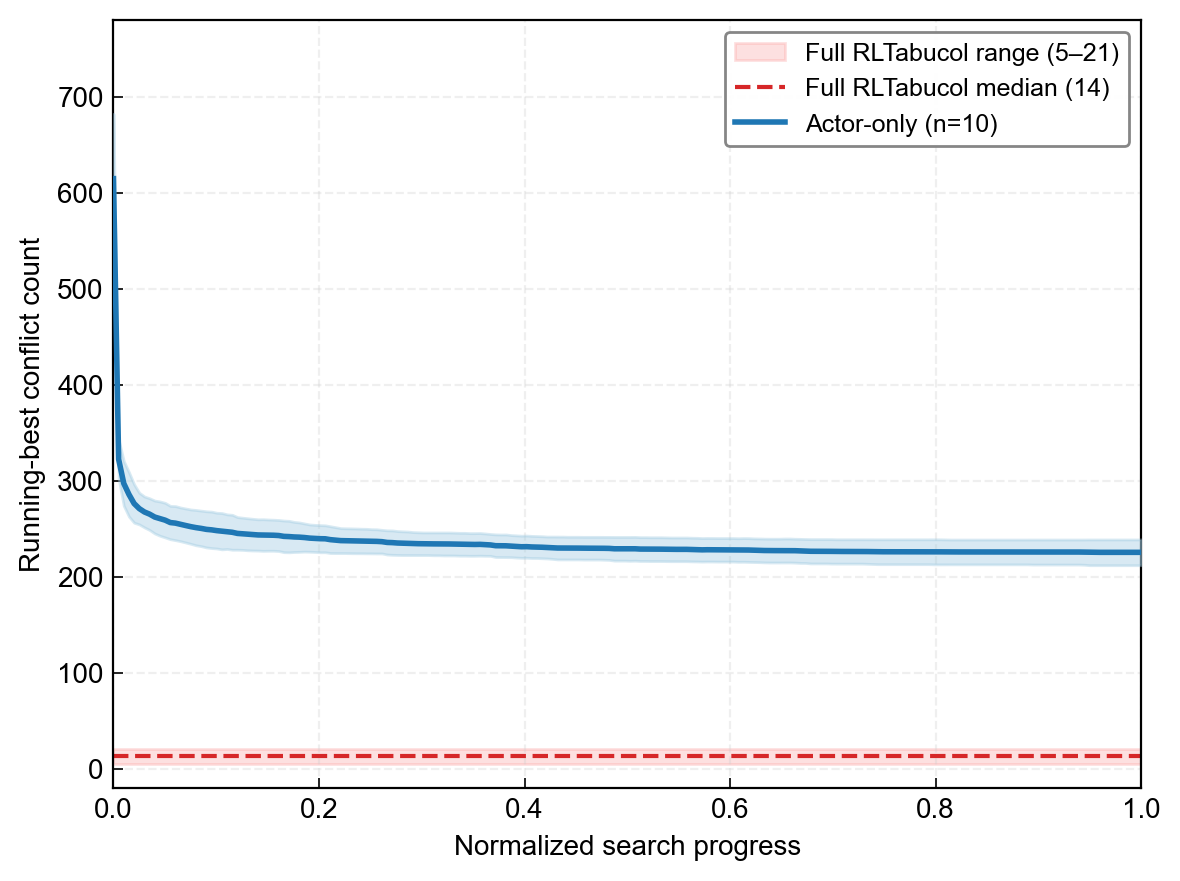
\includegraphics[width=\linewidth]{../figures/generated/actor_only_le45015d.png}
\caption{Actor-only diagnostic on \texttt{le450\_15d} ($k=15$). The actor-only curve summarizes ten runs over normalized search progress; the red band shows the full RLTabucol final range of $5$--$21$ conflicts. Its median of $13.5$ is rounded to $14$ in the legend.}
\label{fig:actor-only-curve}
\end{figure}

\subsection{Cross-framework policy transfer}
\label{ssec:res-rlaco}

Motivated by the actor-only analysis, we next test whether the same frozen policy is more useful when its guidance is consumed by a population-based constructor rather than handed directly to Tabucol. Table~\ref{tab:rlaco-config} reports the results: RLACO$_{\rm soft}$ obtains lower observed best and mean conflicts than both Pure ACO and RLACO$_0$ on all ten instances. Relative to RLACO$_0$, the observed-best reduction ranges from $20$ conflicts on \texttt{le450\_25c} to $154$ on \texttt{DSJC500.9}. Two-sided Welch tests on the ten final conflict values per configuration remain significant after Holm correction on all ten instances, with a largest adjusted $p$-value of $0.00122$. The three source-framework failure cases are particularly informative.
Relative to RLACO$_0$, RLACO$_{\rm soft}$ reduces the observed best from
$150$ to $58$ on \texttt{flat300\_28\_0}, from $295$ to $222$ on
\texttt{le450\_15c}, and from $290$ to $229$ on \texttt{le450\_15d}.
These values remain nonzero, so the transfer stage does not recover legal
colorings at the tested color budgets. Nevertheless, the same frozen policy
that underperforms random guidance on these instances in the source
RLTabucol framework yields lower residual conflicts than RLACO$_0$ when
its learned preferences are used to guide ACO. Overall, these results suggest that policy
usefulness depends not only on the learned guidance itself, but also on how
that guidance is used by the surrounding search framework.

The comparison with RLACO$_{\rm config}$ focuses more directly on the transferred prior. RLACO$_{\rm soft}$ achieves a lower observed best on six instances, ties on \texttt{DSJC500.9}, and is worse on three. Two of the three losses are only one conflict, on \texttt{flat300\_28\_0} and \texttt{le450\_15c}. On the tied \texttt{DSJC500.9} case, RLACO$_{\rm soft}$ also has a lower mean and standard deviation ($47.4\pm3.4$ versus $48.4\pm3.9$). In the other direction, the learned prior improves the observed best by $17$ conflicts on both \texttt{le450\_25c} ($43$ versus $60$) and \texttt{le450\_25d} ($44$ versus $61$), and by $9$ on \texttt{DSJC500.1} ($48$ versus $57$). Although it does not win on every instance, the learned prior is stronger overall than the conflict-constructed prior: it wins more often than it loses, and several of its gains are substantially larger than its small losses.

\begin{table*}[t]
\centering
\caption{Transfer comparison at fixed tested $k$. Entries are best conflicts (mean$\pm$sample standard deviation); the lowest best value per row is bold, including ties. All cells contain ten complete runs. RLACO$_0$ is the random-policy transfer reference defined in Section~\ref{ssec:rlaco}. Welch $t$ uses RLACO$_0$ minus RLACO$_{\rm soft}$, with ten runs per group; two-sided $p$-values are Holm-adjusted across ten instances.}
\label{tab:rlaco-config}
\setlength{\tabcolsep}{3pt}
\resizebox{\textwidth}{!}{\begin{tabular}{@{}lccccccc@{}}
\toprule
Instance & $\chi/k^\star$ & $k$ & Pure ACO & RLACO$_0$ (hard) & RLACO$_{\rm config}$ & RLACO$_{\rm soft}$ & Welch $t$\\
\midrule
\texttt{DSJC250.5} & ?/28 & 28 & 69 (74.6$\pm$3.5) & 70 (76.6$\pm$2.9) & 21 (24.7$\pm$2.8) & \textbf{16 (22.7$\pm$3.1)} & 39.7 \\
\texttt{DSJC500.1} & ?/12 & 12 & 123 (134.2$\pm$6.1) & 136 (141.4$\pm$2.3) & 57 (65.7$\pm$6.9) & \textbf{48 (62.9$\pm$11.6)} & 21.0 \\
\texttt{DSJC500.5} & ?/47 & 48 & 224 (229.9$\pm$3.1) & 225 (230.0$\pm$3.6) & 76 (84.7$\pm$6.9) & \textbf{74 (78.1$\pm$3.4)} & 97.9 \\
\texttt{DSJC500.9} & ?/126 & 126 & 192 (194.9$\pm$2.8) & 196 (202.1$\pm$3.0) & \textbf{42 (48.4$\pm$3.9)} & \textbf{42 (47.4$\pm$3.4)} & 110.3 \\
\texttt{flat300\_26\_0} & 26/26 & 26 & 179 (187.8$\pm$5.0) & 187 (194.7$\pm$3.6) & \textbf{86 (92.9$\pm$4.9)} & 93 (96.7$\pm$4.9) & 50.9 \\
\texttt{flat300\_28\_0} & 28/28 & 28 & 136 (145.5$\pm$4.8) & 150 (155.6$\pm$2.6) & \textbf{57 (62.3$\pm$4.1)} & 58 (62.4$\pm$3.1) & 73.4 \\
\texttt{le450\_15c} & 15/15 & 15 & 293 (297.6$\pm$2.4) & 295 (298.0$\pm$1.6) & \textbf{221 (237.0$\pm$10.7)} & 222 (244.0$\pm$13.1) & 24.9 \\
\texttt{le450\_15d} & 15/15 & 15 & 295 (300.8$\pm$2.6) & 290 (301.4$\pm$5.3) & 234 (254.5$\pm$13.6) & \textbf{229 (249.2$\pm$13.2)} & 11.6 \\
\texttt{le450\_25c} & 25/25 & 25 & 68 (70.3$\pm$1.7) & 63 (68.0$\pm$2.7) & 60 (62.9$\pm$2.4) & \textbf{43 (57.2$\pm$6.9)} & 4.7 \\
\texttt{le450\_25d} & 25/25 & 25 & 70 (72.2$\pm$1.4) & 66 (70.0$\pm$1.7) & 61 (64.7$\pm$2.4) & \textbf{44 (50.5$\pm$6.4)} & 9.2 \\
\bottomrule
\end{tabular}
}
\end{table*}

To examine how the transferred guidance is used inside RLACO, Figure~\ref{fig:rl_aco_share} reports the positive conflict reduction recorded in the RL and ACO phases. On the random and flat graphs, the RL phase accounts for $91.2\%$--$99.3\%$ of the cumulative positive reduction, while the shares on \texttt{le450\_15c} and \texttt{le450\_15d} fall to $72.1\%$ and $66.7\%$. The pattern changes sharply on \texttt{le450\_25c} and \texttt{le450\_25d}, where the RL shares are only $0.45\%$ and $0.84\%$, yet RLACO$_{\rm soft}$ still gives the strongest observed transfer results on those instances. This is important because it shows that the policy's useful behavior is not limited to conflicts removed directly during the RL phase. On some graphs the policy acts mainly as a direct reducer; On other instances, the policy's color distribution mainly acts as a construction bias, helping ACO generate lower-conflict candidate colorings. This pattern also indicates that the policy's utility is not limited to conflicts
removed directly during the RL phase; its learned color preferences can also
provide useful search bias to the subsequent ACO construction.

Overall, the soft-injection interface transfers useful policy information across frameworks. It consistently improves on unguided and random-policy ACO, is stronger overall than the explicit conflict-constructed prior, and remains useful even when the RL phase itself contributes little direct conflict reduction. These results motivate retaining the learned soft prior for the terminal optimization experiment.

\begin{figure*}[t]
\centering
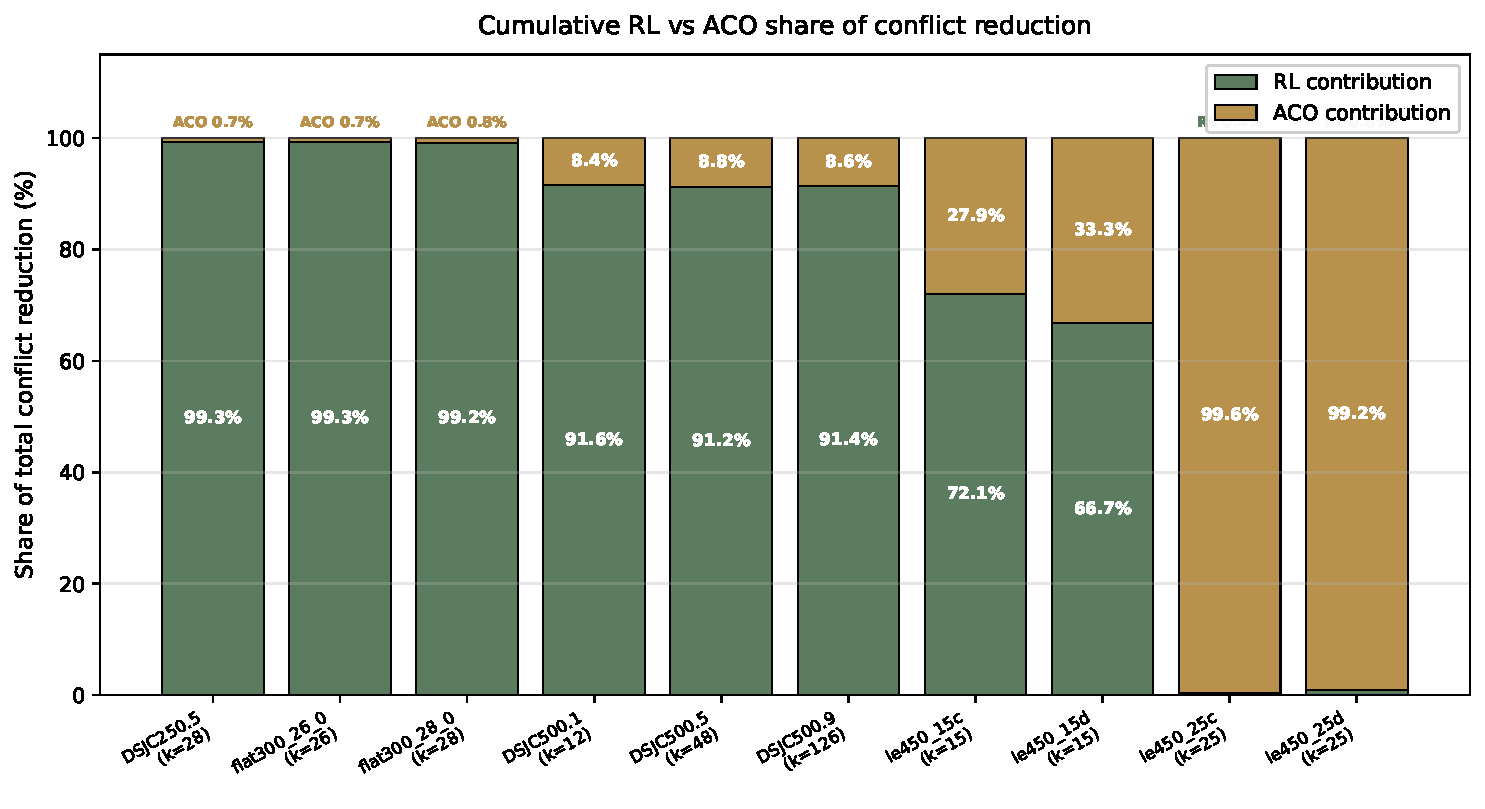
\includegraphics[width=0.85\linewidth]{../figures/generated/component_analysis_vertical.pdf}
\caption{Cumulative shares of positive conflict reduction recorded during the RL and ACO phases across ten transfer instances. The phase-share metric is defined in Section~\ref{ssec:rlaco}.}
\label{fig:rl_aco_share}
\end{figure*}

\subsection{Optimization with RLACO-initialized Tabucol}
\label{ssec:terminal}

The transfer results show that the learned soft prior improves ACO even when the source RLTabucol coupling is inconsistent. We therefore make one final step: use RLACO to prepare the starting coloring for the downstream Tabucol local solver. In RLACO$\rightarrow$Tabucol, the RLACO stage uses the same instance-specific preparation budget as in Section~\ref{ssec:res-rlaco}; its best coloring is then handed to the same Tabucol solver used in the Pure Tabucol baseline. As defined in Section~\ref{ssec:terminal-method}, the reported time starts at this handoff because the timing experiment measures how efficiently Tabucol exploits the prepared initialization.

The results show that RLACO$\rightarrow$Tabucol improves both attainable solution quality and the downstream Tabucol refinement profile. It reaches a lower $k_{\mathrm{best}}$ than Pure Tabucol on five instances and ties it on the other six. Relative to RLTabucol it again records five wins and six ties, and the same $5$--$6$--$0$ win--tie--loss profile holds against RLTabucol$_0$. RLACO$\rightarrow$Tabucol is therefore best or tied for best on all eleven instances. Two cases are strictly better than all three comparators: \texttt{DSJC500.9}, where it reaches $k=126$ instead of $128$, $128$, and $130$, and \texttt{le450\_25d}, where it reaches $k=25$ instead of $26$ for all three source methods. The three instances on which RLTabucol underperformed RLTabucol$_0$ are all recovered at the terminal stage. On \texttt{le450\_15c} and \texttt{le450\_15d}, RLACO$\rightarrow$Tabucol reaches $k=15$ rather than the RLTabucol value of $16$; on \texttt{flat300\_28\_0}, it reaches $k=30$ rather than $31$. The \texttt{DSJC500.9} result gives the clearest link between transfer and optimization: RLACO$_{\rm soft}$ first reduces the fixed-$k=126$ residual to an observed best of $42$ conflicts without local search, after which the downstream Tabucol stage reaches a legal $126$-coloring. The three source methods reach only $128$, $128$, and $130$ colors.

\begin{table*}[t]
\centering
\caption{Terminal optimization comparison. Each method reports its attained $k_{\rm best}$, the number of successful runs out of ten, and best / mean time in seconds over successful runs only. Bold $k_{\rm best}$ values are the lowest per row, including ties. Best and mean times are compared and bolded independently only among methods attaining that row-minimum color budget; times from methods reported at larger $k$ are shown for completeness but are not used for cross-method speed claims. For RLACO$\rightarrow$Tabucol, timing starts at the RLACO-to-Tabucol handoff.}
\label{tab:terminal-comparison}
\setlength{\tabcolsep}{2.1pt}
\resizebox{\textwidth}{!}{% Time is best / mean over successful runs only.
% NOTE: flat300_26_0 RLTabucol mean is set to 1147.8 to match the source-framework table;
% a legacy terminal-time table contained 772.6 and should be checked against raw logs before submission.
\begin{tabular}{@{}lcccccccccccc@{}}
\toprule
Instance & \multicolumn{3}{c}{Pure Tabucol} & \multicolumn{3}{c}{RLTabucol} & \multicolumn{3}{c}{RLTabucol$_0$} & \multicolumn{3}{c}{RLACO$\rightarrow$Tabucol}\\
 & $k_{\rm best}$ & Success & Time (s) & $k_{\rm best}$ & Success & Time (s) & $k_{\rm best}$ & Success & Time (s) & $k_{\rm best}$ & Success & Time (s)\\
\midrule
\texttt{DSJC250.5} & \textbf{28} & 10/10 & 14.6 / 45.5 & \textbf{28} & 10/10 & 243.8 / 3046.5 & \textbf{28} & 10/10 & 2.6 / 269.0 & \textbf{28} & 9/10 & \textbf{1.5} / \textbf{36.5} \\
\texttt{DSJC500.1} & \textbf{12} & 7/10 & 2356.2 / 6001.4 & \textbf{12} & 8/10 & \textbf{936.9} / \textbf{3616.9} & 13 & 10/10 & 0.4 / 0.6 & \textbf{12} & 9/10 & 1358.0 / 4994.4 \\
\texttt{DSJC500.5} & \textbf{49} & 10/10 & \textbf{408.5} / \textbf{1519.6} & \textbf{49} & 6/10 & 2375.5 / 7664.3 & 50 & 10/10 & 101.9 / 1303.2 & \textbf{49} & 10/10 & 424.0 / 1755.7 \\
\texttt{DSJC500.9} & 128 & 8/10 & 2513.0 / 8521.6 & 128 & 4/10 & 3062.7 / 8749.3 & 130 & 7/10 & 1080.5 / 4289.1 & \textbf{126} & 1/10 & \textbf{7330.6} / \textbf{7330.6} \\
\texttt{le450\_15c} & 16 & 10/10 & 0.2 / 45.2 & 16 & 10/10 & 4.1 / 246.7 & \textbf{15} & 10/10 & 273.1 / 1283.2 & \textbf{15} & 2/10 & \textbf{130.8} / \textbf{252.0} \\
\texttt{le450\_15d} & 16 & 9/10 & 0.3 / 302.5 & 16 & 10/10 & 32.2 / 1085.3 & \textbf{15} & 9/10 & 932.4 / 6956.8 & \textbf{15} & 1/10 & \textbf{578.5} / \textbf{578.5} \\
\texttt{le450\_25c} & \textbf{26} & 9/10 & 5.4 / 12.4 & \textbf{26} & 10/10 & 44.7 / 141.0 & \textbf{26} & 10/10 & 3.3 / 16.5 & \textbf{26} & 10/10 & \textbf{1.5} / \textbf{7.4} \\
\texttt{le450\_25d} & 26 & 10/10 & 7.6 / 14.5 & 26 & 10/10 & 44.8 / 106.6 & 26 & 10/10 & 1.9 / 17.5 & \textbf{25} & 2/10 & \textbf{8480.7} / \textbf{8771.6} \\
\texttt{flat300\_26\_0} & \textbf{26} & 10/10 & \textbf{8.8} / 215.8 & \textbf{26} & 10/10 & 229.2 / 1147.8 & \textbf{26} & 10/10 & 134.3 / 704.4 & \textbf{26} & 10/10 & 13.3 / \textbf{167.9} \\
\texttt{flat300\_28\_0} & \textbf{30} & 1/10 & 9453.8 / 9453.8 & 31 & 10/10 & 150.4 / 1278.2 & \textbf{30} & 1/10 & 14021.1 / 14021.1 & \textbf{30} & 1/10 & \textbf{4788.2} / \textbf{4788.2} \\
\texttt{flat1000\_76\_0} & 88 & 1/10 & 16485.4 / 16485.4 & \textbf{87} & 1/10 & \textbf{8920.2} / \textbf{8920.2} & 90 & 10/10 & 303.9 / 1349.2 & \textbf{87} & 1/10 & 13323.9 / 13323.9 \\
\bottomrule
\end{tabular}
}
\end{table*}

The timing results show that the improved initialization is often easier for the downstream Tabucol solver to exploit. Among methods that attain the row-minimum $k_{\mathrm{best}}$, RLACO$\rightarrow$Tabucol has the shortest best successful-run refinement time on seven of eleven instances and the shortest mean successful-run time on eight. Two of those rows, \texttt{DSJC500.9} and \texttt{le450\_25d}, are cases in which RLACO$\rightarrow$Tabucol alone reaches the best color budget. Excluding them gives a stricter shared-target comparison: RLACO$\rightarrow$Tabucol remains fastest on five of nine instances by best successful time and six of nine by mean successful time. This improvement is not explained simply by handing Tabucol a lower-conflict coloring. The original RLTabucol pipeline already presents Tabucol with states after substantial policy-driven conflict reduction, yet it does not consistently outperform Pure Tabucol; the transfer stage changes how the learned information is organized before the downstream handoff.

Success counts provide a complementary measure of reliability, but they must be interpreted at the color budget being attempted. A lower $k$ defines a harder fixed-$k$ problem, so success rates reported at different color budgets are not directly comparable. At the new frontiers, RLACO$\rightarrow$Tabucol succeeds in $1/10$ runs at $k=126$ on \texttt{DSJC500.9} and at $k=15$ on \texttt{le450\_15d}, and in $2/10$ runs on \texttt{le450\_15c} and \texttt{le450\_25d}. At shared targets the pattern is stronger: on \texttt{DSJC500.1} at $k=12$, it succeeds in $9/10$ runs, compared with $8/10$ for RLTabucol and $7/10$ for Pure Tabucol; on \texttt{DSJC500.5} at $k=49$, it reaches $10/10$, matching Pure Tabucol and exceeding RLTabucol's $6/10$. Because solution quality is determined first by the attained color budget, success rate is treated as a secondary reliability measure rather than the primary measure of optimization performance.

Overall, RLACO$\rightarrow$Tabucol converts the cross-framework transfer result into the intended optimization gain. The staged framework reaches equal or better color quality on every tested instance and, once the RLACO initialization is available, gives the downstream Tabucol solver the strongest overall refinement-time profile. The contribution is therefore not limited to transferring a policy between frameworks: the transferred policy is used to construct an initialization that improves both attainable solution quality and downstream solving efficiency.
